\documentclass{article}
\usepackage{amsmath,amssymb,amsfonts}
\usepackage{latexsym}
\usepackage{graphicx}
\usepackage{verbatim}
\usepackage{booktabs}
\usepackage[usenames,dvipsnames,svgnames,table]{xcolor}
\usepackage{todonotes} % Required for the boxes that questions appear in
\newcommand{\mybox}[1]
{
\par\noindent
\todo[inline, backgroundcolor=SkyBlue!40,bordercolor=SkyBlue,size=\large]{\textbf{#1}}
\vspace{1em}
}

\usepackage[top=25mm, bottom=25.4mm, left=16.7mm, right=18.9mm]{geometry}

\usepackage{fancyhdr}
\pagestyle{fancy}
\lhead{Numerical Analysis Assignment \#2 }
\chead{Xinglu Wang \quad 3140102282}
\renewcommand{\headrulewidth}{0.3pt}

\usepackage[framed,numbered,autolinebreaks,useliterate,final]{mcode}

\title{\textbf{Numerical Analysis Assignment \#2}}
\author{Xinglu Wang \qquad Student Number: 3140102282
    \\ %\vspace{0.5em}
    College of Information Science \& Electronic Engineering}
\date{}

\usepackage{sectsty}
\subsectionfont{\color{NavyBlue!90}\itshape\selectfont}
\makeatletter
\newcommand{\sectbox}[1]{%
\noindent\protect\fbox{%
\@tempdima=\hsize
\advance\@tempdima by-2\fboxsep
\advance\@tempdima by-2\fboxrule
\protect\parbox{\@tempdima}{
\fcolorbox{SkyBlue}{NavyBlue!80}{\parbox{\linewidth -2\fboxsep -2\fboxrule}{
\color{white}{#1}
}}
}}}
\makeatother
\sectionfont{\sectbox}

\makeatletter
\def\@seccntformat#1{%
  \expandafter\ifx\csname c@#1\endcsname\c@section\else
  \csname the#1\endcsname\quad
  \fi}
\makeatother

\newcommand{\abs}[1]{\left| #1 \right| }

\usepackage{multirow}

\begin{document}
\maketitle

\section{Problem 1}
According to Newton's method, $g(x)=x-\frac{f(x)}{f'(x)}$. We get
\begin{equation}%\lable{}
    g(x)=x+\frac{cosx+x^3}{sinx-3x^2}
\end{equation}


Using $g(x)=x$ to iterate, We get iteration point shown below:
\begin{center}
    \begin{tabular}{c}
        \toprule
        Iteration Point\\
        \midrule
        -1.000000000000000\\
        \midrule
        -0.880332899571582\\
        \midrule
        -0.865684163176082\\
        \bottomrule
    \end{tabular} \\ \vspace{10pt}
    Table 1.1 Data for problem 1\\ \vspace{10pt}
    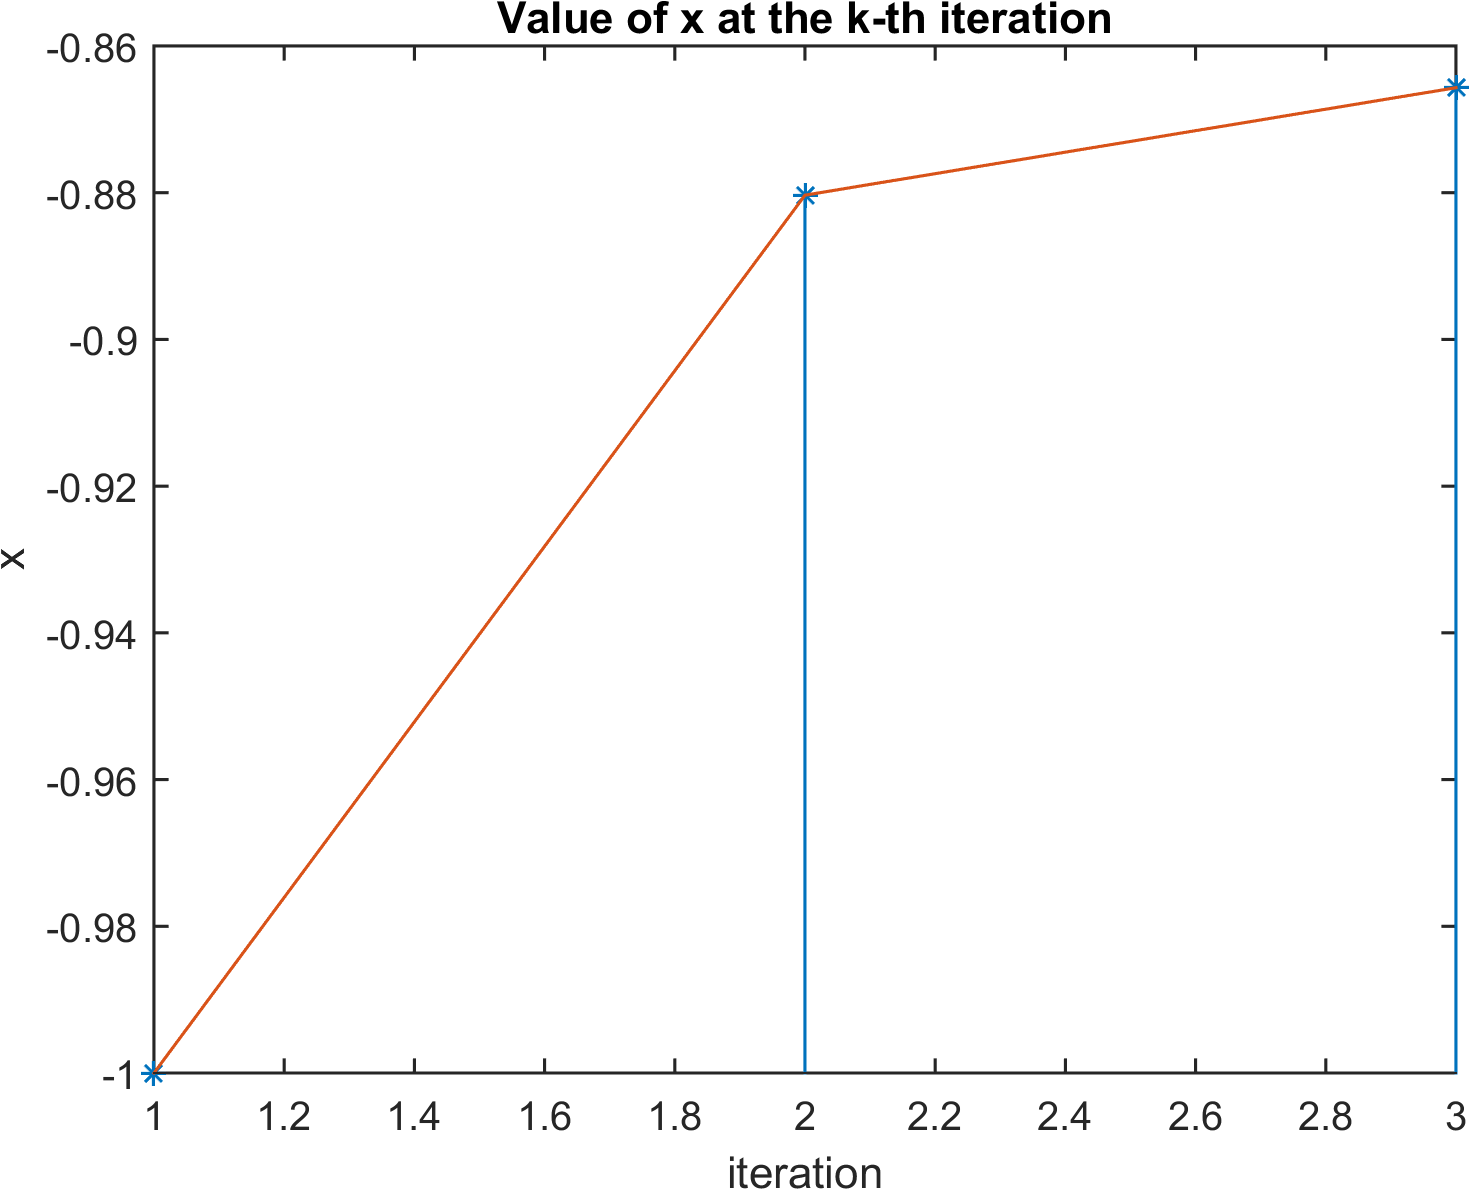
\includegraphics[height=6.5cm]{../pic/q1_1.png}\\
    Figure 1.1 Plot point for problem 1
\end{center}
Therefore, $p_2=-0.865684163176082$ \\
  And $p_0 \text{ should not be } 0$, otherwise $f'(p_0)$ would be $0$, and we cannot get an appropriate $p_1$.\\
The usage of Implement of Newton's method is shown below:
\begin{lstlisting}
    %% problem 1
    format long;
    clear
    f1=@(x) -x^3-cos(x);
    Newton(f1,-1,10^-5,2);
\end{lstlisting}

The Implement of Newton's method is shown below:
\lstinputlisting{../mcode/Newton.m}

Refer to code ��Problem1.m��.
When p0 = -1, we get p2 = -0.865684163176082.


\section{Problem 2}
\begin{description}
  \item[i).]
  According to Newton-Raphson method, $x_{k+1}=x_k-\frac{f(x_k)}{f'(x_k)} \quad \text{,where } k \in \mathbb{N} $. We infer that
\begin{equation}
x_{k+1}=2x_k-b{x_k}^2
\end{equation}
Since $\varepsilon_k=\frac{\frac{1}{b}-x_k}{\frac{1}{b}}$, we infer that
\begin{equation}
{\abs{\varepsilon _{k + 1}}} = \frac{{\frac{1}{b} - {x_{k + 1}}}}{{\frac{1}{b}}} = {(1 - b{x_k})^2} = { {{\varepsilon _k}} ^2}
\end{equation}
  \item[ii).]
  When $0<x_0<\frac{2}{b}$, $\varepsilon_0=\frac{\frac{1}{b}-x_0}{\frac{1}{b}}<1 $, according to \textbf{i).}, $\{\varepsilon_k\}$ is a geometric progression series whose common ratio is below 1. So the relative error $\varepsilon_k \rightarrow 0$, and $x \rightarrow \frac{1}{b}$
\end{description}


\section{Problem 3}
\begin{description}
  \item[a).]
  \begin{eqnarray*}
    3x_1-cos(x_1x_2)-\frac{1}{2} &=& 0 \\
    4{x_1}^2-625{x_2}^2+2x_2-1 &=& 0 \\
    \mathrm{e}^{-x_1x_2}+20x_3+\frac{10\pi-3}{3} &=& 0
  \end{eqnarray*}
    After running the code,we get x of each iteration.\\
  \begin{center}
    \begin{tabular}{ccc}
      \toprule
      initial & first iter & second iter \\ \midrule
       0 &   0.500000000000000 &   0.500166686911463\\ \midrule
       0 &   0.500000000000000 &   0.250803638439239\\ \midrule
       0 &  -0.523598775598299 &  -0.517387427392491\\ \bottomrule
    \end{tabular}
   \end{center}
   Thus the answer $x_2$ is \[{x_2} = \left\{ {\begin{array}{*{20}{c}}
{{\rm{0}}{\rm{.500166686911463}}}\\
{{\rm{0}}{\rm{.250803638439239}}}\\
{{\rm{ - 0}}{\rm{.517387427392491}}}
\end{array}} \right\}\]
	The usage of Implement of Newton's method for nonlinear equation system is shown below:
	\begin{lstlisting}
%% problem 3
clear
format long;
syms f1 f2;
x=sym('x',[3,1]);
f1=[3*x(1)-cos(x(2)*x(3))-1/2;...
    4*x(1)^2-625*x(2)^2+2*x(2)-1;...
    exp(-x(1)*x(2))+20*x(3)+(10*pi-3)/3];
%MetrixPlot(f1(1));
f2=[x(1)^2+x(2)-37;...
    x(1)-x(2)^2-5;...
    x(1)+x(2)+x(3)-3];
NewtonNonlin(f1,x,[0,0,0].',2)
NewtonNonlin(f2,x,[0,0,0].',2)
	\end{lstlisting}
	
	Implement of Newton's method for nonlinear equation system is shown below:
	\lstinputlisting{../mcode/NewtonNonlin.m}
    I still have many thing to optimize, this implement is not robust and can not be applied into common use. There are many skill to deal with matrix in math, but I am not experienced enough.
  \item[b).]
  Similarly, we get x for each iteration shown below
  \begin{center}
    \begin{tabular}{ccc}\toprule
                    initial & first iter & second iter \\ \midrule
                   0 &   5.000000000000000 &   4.350877192982456\\
                   0 &  37.000000000000000 &  18.491228070175438\\
                   0 & -39.000000000000000 & -19.842105263157897\\\bottomrule
     \end{tabular}
  \end{center}
  Thus the answer is \[{x_2} = \left\{ {\begin{array}{*{20}{c}}
{{\rm{4}}{\rm{.350877192982456}}}\\
{{\rm{18}}{\rm{.491228070175438}}}\\
{{\rm{ - 19}}{\rm{.842105263157897}}}
\end{array}} \right\}\]
\end{description}
\section{Problem 4}
\begin{description}
  \item[a).]
  Although Steepest Descent method is not as strict  with initial value as Newton method for nonlinear system, it still need a estimation for initial value. (It is apparent by thinking the gradient decides where this points will go in next iteration.) So I use the matlab function \textbf{solve} to find symbolic answer for this problem, then add initial estimation for my programme. The way for prediction is shown below
  \begin{lstlisting}
%%for estimating and predicting
[x1,x2,x3]=solve([f1==0,f2==0,f3==0]);
for ii=1:size(x1,1)
    res=[];
    for jj=1:3
        tmp=eval(['x',num2str(jj)]);
        tmp2=tmp(ii);
        res=[res;tmp2];
    end
    disp(double(res));
end
	\end{lstlisting}
The result is show below,\\

\begin{center}
   \begin{tabular}{|c|c|}
		  \hline
           \multirow{3}[6]*{solution 1}
                    & $  -8.441429707360641   $\\\cline{2-2}
                   & $  -7.940157258463179 $\\\cline{2-2}
                   & $  -19.143837080321028 $\\
           \hline
          \multirow{3}[6]*{solution 2}
                    & $  1.036400470329211   $\\\cline{2-2}
                   & $  1.085706550741678 $\\\cline{2-2}
                   & $ 0.931191442315390 $\\
           \hline
           \multirow{3}[6]*{solution 3}
                    &   $8.708234096655289 + 6.936510819683741i  $ \\\cline{2-2}
                   &  $-0.793852371079888 - 9.117849140990071i $ \\\cline{2-2}
                   &  $8.779635019761287 +29.631028653675870i$\\
           \hline
           \multirow{3}[6]*{solution 4}
                    & $  0.619280521860425 + 8.523979282877251i   $\\\cline{2-2}
                   & $  10.471077724940638 + 4.493153163724587i $\\\cline{2-2}
                   & $  21.436062799241533 +55.489000314501233i$\\
           \hline
           \multirow{3}[6]*{solution 5}
                    & $   8.708234096655289 - 6.936510819683741i  $\\\cline{2-2}
                   & $  -0.793852371079888 + 9.117849140990071i $\\\cline{2-2}
                   & $  8.779635019761287 -29.631028653675870i$\\
           \hline
           \multirow{3}[6]*{solution 6}
                    & $   0.619280521860425 - 8.523979282877251i  $\\\cline{2-2}
                   & $  10.471077724940638 - 4.493153163724587i $\\\cline{2-2}
                   & $ 21.436062799241533 -55.489000314501233i $\\
           \hline

    \end{tabular}
\end{center}

From the result we can know that every method has its privilege and inferiority.
Steepest method still depends on initial value, We can conclude that

\begin{center}
\noindent\fcolorbox{SkyBlue}{SkyBlue!30}{\parbox{\linewidth -2\fboxsep -2\fboxrule}{
   \begin{tabular}{c|l}
		  \hline
           \multirow{1}[2]*{Advantage}
                    &  No matter what initial value we give it, as long as gradient is not $0$, it will converge. \\
           \hline
           \multirow{2}[5]*{Disadvantage} &  It determines a local minimum
for a multivariable function.\\\cline{2-2}
                   & It converges only linearly to the
solution \\\cline{2-2}
                     & Unlike symbolic method, it cannot give complex answer such as $a+bi$ \\\cline{2-2}
                   &  If we choose a bad alpha, it will become quite slow. \\
           \hline
    \end{tabular}
    }}
\end{center}

And my answer is shown below. Compared with the answer calulated by matlab, my answer is quite accurate in the terms of $TOL=0.05$. When I choose $TOL=10^{-5}$ and find that if TOL become smaller, then size of step should also be smaller.To sum up, size of step ,max iteration times, tolerance are closely related. I have not tried the self-adaptation method for calculate $\alpha$. If it is applied,I think, it can calculate more fast but no more accurate, since I have chosen a small step size.
\begin{center}
   \begin{tabular}{|c|c|}
		  \hline
           \multirow{3}[6]*{solution $ x_1 \in \mathbb{R} $}
                    &  1.036498009046320   \\\cline{2-2}
                   &  1.085380893216069\\\cline{2-2}
                   &  0.931139784999289 \\
           \hline
          \multirow{3}[6]*{solution $x_2 \in \mathbb{R}$}
                    &   -8.440255795243777 \\\cline{2-2}
                   &  -7.939370693306589 \\\cline{2-2}
                   & -19.137864730324921 \\
           \hline
    \end{tabular}
\end{center}
The usage of Steepest Descent method is shown below,
\begin{lstlisting}
% problem 4
clear
format long
syms x1 x2 x3 f1 f2 f3 g1 g2;
f1=15*x1+x2^2-4*x3-13;
f2=x1^2+10*x2-x3-11;
f3=x2^3-25*x3+22;
g1=f1^2+f2^2+f3^2;
x=[x1;x2;x3];
tol=10^-5;
MaxIter=10000;

ini=[1;1;1];
res=SDescent(g1,x,ini,tol,MaxIter);
disp(res(:,end));

ini=[-8,-8,-19];
res=SDescent(g1,x,ini,tol,MaxIter);
disp(res(:,end));

f1=10*x1-2*x2^2+x2-2*x3-5;
f2=8*x2^2+4*x3^2-9;
f3=8*x2*x3+4;
g2=f1^2+f2^2+f3^2;

ini=[1;0;1];
res=SDescent(g2,x,ini,tol,MaxIter);
disp(res(:,end));

ini=[0,1,-1];
res=SDescent(g2,x,ini,tol,MaxIter);
disp(res(:,end));

ini=[1,-1,0];
res=SDescent(g2,x,ini,tol,MaxIter);
disp(res(:,end));

ini=[0,0,-1];
res=SDescent(g2,x,ini,tol,MaxIter);
disp(res(:,end));
\end{lstlisting}
The implement of Steepest Descent method is shown below, and we will see there are munch space to improve our implement to make the programme more robust.
\lstinputlisting{../mcode/SDescent.m}

  \item[b).]
    Similarly, via estimating first and applying Steepest Descent method, We can get 
\begin{center}
   \begin{tabular}{|c|c|}
		  \hline
           \multirow{3}[6]*{$ x_1 \in \mathbb{R} $}
                    &    0.843203979094425 \\\cline{2-2}
                   &  -0.353845516901669\\\cline{2-2}
                   &   1.413882789399937\\
           \hline
            \multirow{3}[6]*{$ x_2 \in \mathbb{R} $}
                    &   0.497133950969613  \\\cline{2-2}
                   & 0.997545468636543 \\\cline{2-2}
                   &  -0.505700092951828 \\
           \hline
            \multirow{3}[6]*{$ x_3 \in \mathbb{R} $}
                    &   0.900005537385528  \\\cline{2-2}
                   &  -1.000190835623339\\\cline{2-2}
                   &  0.499540078284082 \\
           \hline   
            \multirow{3}[6]*{$ x_4 \in \mathbb{R} $}
                    &   0.206590365596643  \\\cline{2-2}
                   & 0.353736566702580\\\cline{2-2}
                   & -1.414033729757102  \\
           \hline
    \end{tabular}
\end{center}
\end{description}

\end{document}
